\documentclass[12pt,a4paper]{article}
%
\usepackage[czech]{babel}
\usepackage[utf8x]{inputenc}
\usepackage[T1]{fontenc}
\usepackage{lmodern}
\usepackage[text={14cm,21cm},bottom=5cm]{geometry}
%
\usepackage{amsmath}
\usepackage{graphicx}
\usepackage{verbatim}
\usepackage[colorinlistoftodos]{todonotes}
%
\parindent0pt \parskip8pt
%
\title{Seminární práce }
\author{qwerty2}
%
\begin{document}

\pagenumbering{gobble}% Remove page numbers (and reset to 1)
%
\clearpage
\thispagestyle{empty}
\begin{center}
%

\includegraphics[width=60mm]{pics/favlogo.pdf}
%
\vfill
%
{\large\bf Katedra informatiky / PC}

{\large ŘEŠENÍ KOLIZÍ FREKVENCÍ SÍTĚ VYSÍLAČŮ}

{\large (Semestrální práce)}
%
\vfill
%
\end{center}
%
\vspace{2cm}
%
\begin{tabular}{rl}
student: & Milan Hajžman \\
\noalign{\vspace{2mm}}
studijní číslo: & A13B0303P \\
\noalign{\vspace{2mm}}
email: & qwerty2@students.zcu.cz \\
\noalign{\vspace{2mm}}
datum: & \today \\
\end{tabular}

%
\clearpage
\tableofcontents
\clearpage
%
\pagenumbering{arabic}% Arabic page numbers (and reset to 1)
%
\section{Zadání}
Naprogramujte v ANSI C přenositelnou \textbf{konzolovou aplikaci}, která jako vstup načte z parametru
příkazové řádky název textového souboru obsahující informaci o pozici vysílačů na mapě a na
jeho základě přidělí každému vysílači frekvenci tak, aby jeho signál nekolidoval s vysílači v blízkém
okolí. Úloha je znázorněna obrázku \ref{fig:obrazekzezadani}.

Program se bude spouštět příkazem \texttt{freq.exe} \textit{<soubor-s-vysílači>}. Symbol \textit{<soubor-s-vysílači>}
zastupuje jméno textového souboru, který obsahuje informaci o rozmístění vysílačů na mapě a o
dostupných vysílacích frekvencích, které jim je možné přidělit.
Váš program tedy může být během testování spuštěn například takto:

\texttt{freq.exe vysilace-25.txt}

Výsledkem práce programu bude výpis do konzole se seznamem přidělených frekvencí každému
vysílači ze vstupního souboru (viz Specifikace výstupu programu). V případě chyby nebo
neřešitelné situaci skončí program výpisem příslušné chybové hlášky.

Pokud nebude na příkazové řádce uveden právě jeden argument, vypište chybové hlášení a stručný
návod k použití programu v angličtině podle běžných zvyklostí (viz např. ukázková semestrální
práce na webu předmětu Programování v jazyce C). \textbf{Vstupem programu je pouze argument
na příkazové řádce – interakce s uživatelem pomocí klávesnice či myši v průběhu
práce programu se neočekává.}

Hotovou práci odevzdejte v jediném archivu typu ZIP prostřednictvím automatického odevzdávacího
a validačního systému. Postupujte podle instrukcí uvedených na webu předmětu. Archiv nechť
obsahuje všechny zdrojové soubory potřebné k přeložení programu, makefile pro Windows i Linux
(pro překlad v Linuxu připravte soubor pojmenovaný \texttt{makefile} a pro Windows \texttt{makefile.win})
a dokumentaci ve formátu PDF vytvořenou v typografickém systému \TeX, resp. \LaTeX
. Bude-li některá z částí chybět, kontrolní skript Vaši práci odmítne.

\begin{figure}[htbp]
  \centering
    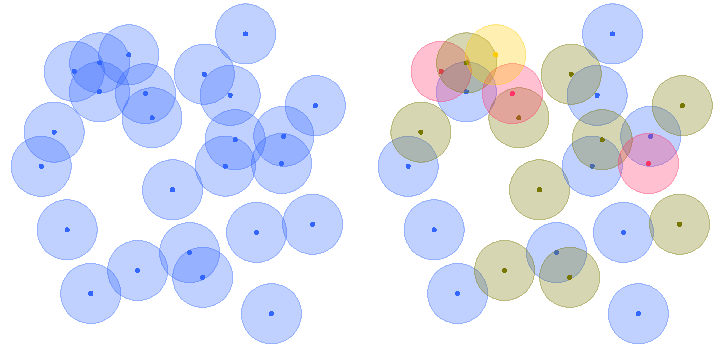
\includegraphics[width=.80\textwidth]{pics/zadaniimg.pdf}
  \caption{Znázornění úlohy. Na mapě je dána množina vysílačů, jejichž pozice je znázorněna
  tečkou. Vysílač dokáže vyslat svůj signál pouze v okruhu do předem definované vzdálenosti. Ve
  skutečnosti spolu ale signály sousedních vysílačů mohou kolidovat (situace vlevo). Každému
  vysílači je proto potřeba přiřadit jinou frekvenci (barvu) tak, aby signál žádné dvojice vysílačů
  nekolidoval (vpravo).}
  \label{fig:obrazekzezadani}
\end{figure}

\newpage
\section{Analýza úlohy}
%
K urychlení procházení sousedních vysílačů je zapotřebí vytvořit graf sousednosti. 
V tomto grafu každá hrana představuje, že se oblasti 
dvou vysílačů překrývají. Taková situace nastane, pokud je vzdálenost mezi dvěma vysílači menší než dvojnásobek
jejich dosahu. Při počtu vysílačů je možno provést kontrolu stylem \uv{každý s každým}. Po kontrole vzdáleností může grafů vzniknout více, 
stejně tak se mohou vyskytovat osamocené vysílače, proto je zapotřebí vícenásobně projít seznam vrcholů a zkontrolovat zda
nezvbývá nenaladěný vysílač.

Počet vysílačů může sahat do tisíců, proto je vhodné graf nedefinovat maticí, 
ale spojovým seznamem nebo polem obsahujícím hrany grafu. Pole je však nevhodné, 
protože dopředu neznáme počet hran, které do nich budeme vkládat. Zároveň jeho výhodu
jít kdykoli na kterýkoli prvek pole nepotřebujeme, protože budeme vždy procházet 
všechny sousední vrcholy.

Při procházení grafu budu potřebovat zásobník, do kterého budu ukládat nenaladěné 
sousední vysílače. Implementuji ho pomocí pole, které v případě potřeby realokuji na větší.

Algoritmus hledání frekvencí je podrobněji popsán UML diagramem na obrázku \ref{fig:uml}.

\begin{figure}[htbp]
  \centering
    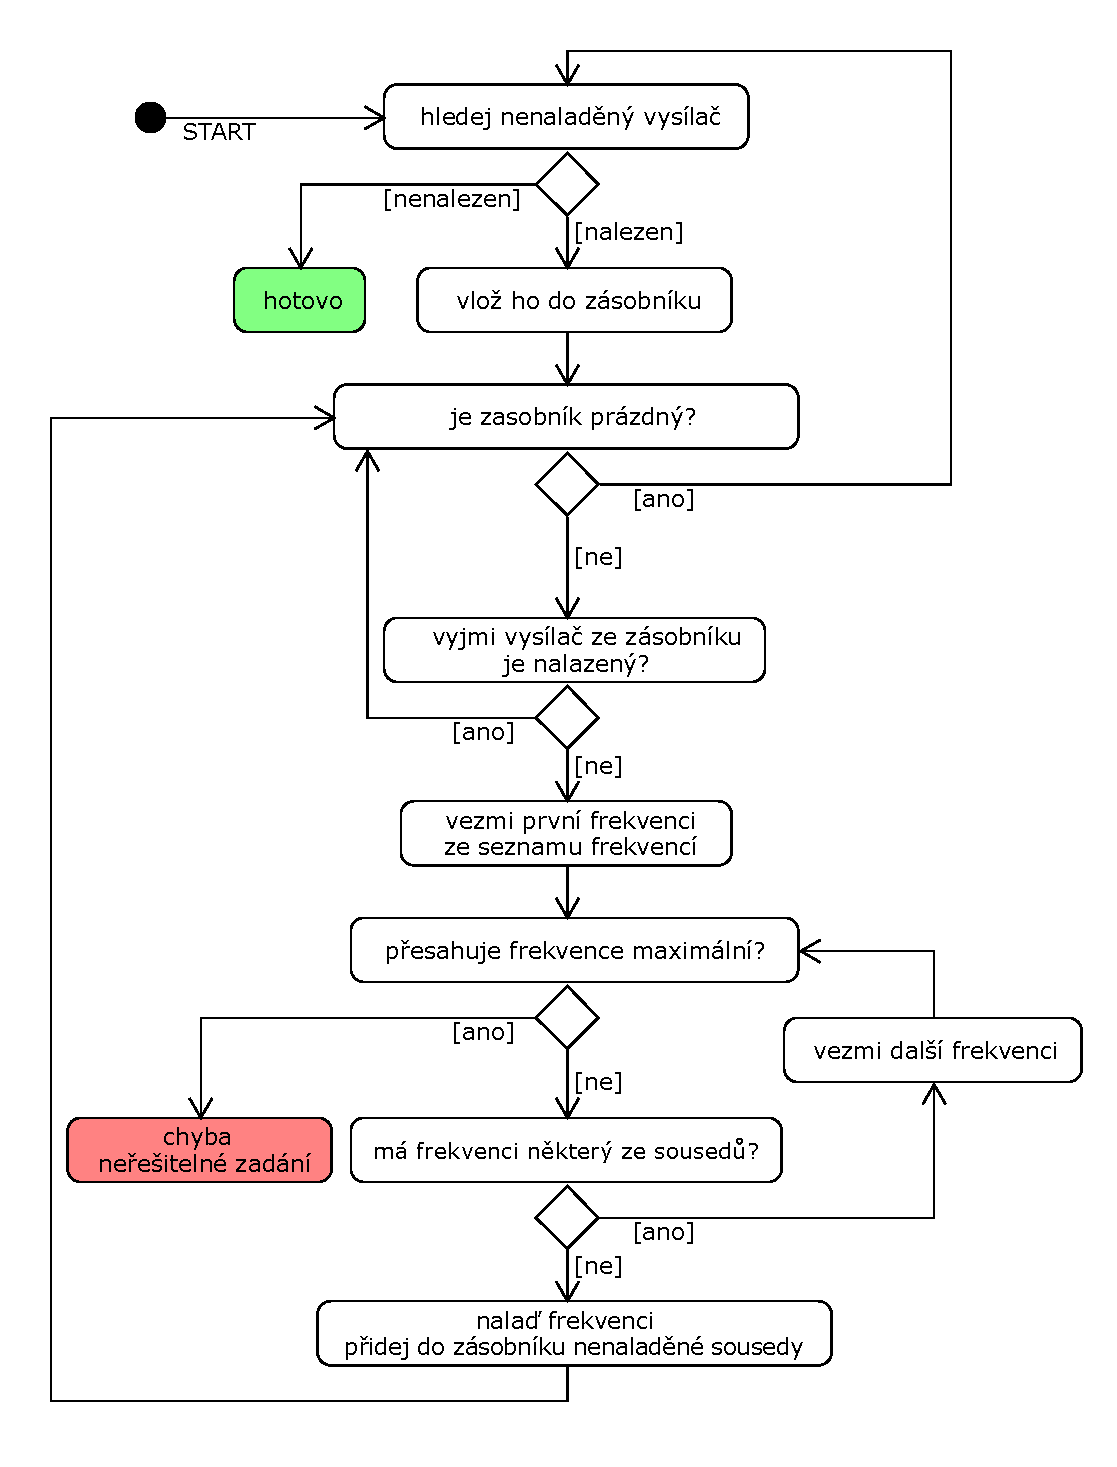
\includegraphics[width=.90\textwidth]{pics/uml.pdf}
  \caption{UML diagram algoritmu pro nalezení nejnižších frekvencí v grafu sousednosti.}
  \label{fig:uml}
\end{figure}
%
\section{Popis implementace}
\subsection {Datové struktury}
\subsubsection {Overlap}
%
Abych nezapomněl nějakou část paměti uvolnit, rozhodl jsem se udržovat vše v jedné struktuře \texttt{Overlap}, 
která bude pointery ukazovat na další struktury, ty pak na dalsí atd. Pak lze kaskádově uvolnit 
všechna naalokovaná místa v paměti jedinou funkcí. \texttt{Overlap} obsahuje počet frekvencí a vysílačů,
dosah vysílačů, pole frekvencí a pole s odkazy na struktury \texttt{Transmitter}.

\begin{verbatim}
typedef struct {

    /* pole s frekvencemi */
    int *freqlist;
    /* dvojity pointer ve smyslu pole ukazatelu na vysilac */
    Transmitter **translist;
    /* delky poli */
    int freqc,translistc;
    /* maximalni vzdalenost mezi dvema vysilaci
     * pri niz dochazi ke kolizi signalu */
    int radius;

} Overlap;
\end{verbatim}

\subsubsection {Transmitter}
Struktura \texttt{Transmitter} představuje jeden vysílač, obsahuje jeho souřadnice,
naladěnou frekvenci a první položku spojového seznamu sousedních vrcholů grafu. Tyto
položky jsou strukturového typu \texttt{Node}. Nenaladěný vysílač má nastavenou
frekvenci rovnající se konstantě \texttt{UNTUNED}. Pokud nemá vysílač žádného souseda,
pak se odkaz na seznam rovná \texttt{NULL}.  

\begin{verbatim}
#define UNTUNED -1

typedef struct {

    /* spojovy seznam sousedu */
    Node *node;
    /* pozice vysilace */
    double x,y;
    /* naladena frekvence, ve smyslu indexu v poli frekvenci */
    int freq;

} Transmitter;
\end{verbatim}

\subsubsection {Node}
Struktura \texttt{Node} obsahuje odkaz na další \texttt{Node} a index vysílače 
v poli vysílačů ve struktuře \texttt{Overlap}. Poslední prvek spojového seznamu ukazuje na \texttt{NULL}.

\begin{verbatim}
typedef struct node {

    /* dalsi polozka */
    struct node *next;
    /* soused - index v poli vysilacu */
    int transmitter;

} Node;
\end{verbatim}

\subsubsection {Intstack}
Struktura \texttt{Intstack} představuje zásobník čísel, který využívám při procházení grafu, 
k upřednostění souseda při dalším ladění frekvencí. Zásobník začne s zadanou velikostí při jeho 
vytvoření. V případě, že hrozí pčtečení, tak se zavolá funkce \texttt{realloc()}, 
která ho zvětší na dvojnásobnou velikost.

\begin{verbatim}
typedef struct {

    /*velikost pole*/
    int stacksize;
    /*pole polozek*/
    int *stack;
    /*vrchol zasobniku*/
    int current_item;

} Intstack;
\end{verbatim}

\subsection{Zdrojové soubory}
\textbf{\texttt{main.c:}} Hlavní zdrojový soubor, obsahuje funkci \texttt{main()} s během 
programu a funkci \texttt{Overlap *load\_file(char *filename)}, která načítá vstupní data 
ze souboru do struktury \texttt{Overlap}.

\textbf{\texttt{overlap.h:}} Obsahuje definici struktury \texttt{Overlap} a prototypy jejích obslužných funkcí.

\textbf{\texttt{overlap.c:}} Obsahuje výkonný kód funkcí ze souboru \texttt{overlap.h}.

\textbf{\texttt{transmitter.h:}} Obsahuje definici struktury \texttt{Transmitter} a prototypy jejích obslužných funkcí.

\textbf{\texttt{transmitter.c:}} Obsahuje výkonný kód funkcí ze souboru \texttt{transmitter.h}.

\textbf{\texttt{node.h:}} Obsahuje definici struktury \texttt{Node} a prototypy jejích obslužných funkcí.

\textbf{\texttt{node.c:}} Obsahuje výkonný kód funkcí ze souboru \texttt{node.h}.

\textbf{\texttt{intstack.h:}} Obsahuje definici struktury \texttt{Intstack} a prototypy jejích obslužných funkcí.

\textbf{\texttt{intstack.c:}} Obsahuje výkonný kód funkcí ze souboru \texttt{intstack.h}.

\textbf{\texttt{errors.h:}} Obsahuje čísla chybových stavů a jejich hlášky.

\textbf{\texttt{errors.c:}} Obsahuje funkci pro předčasné ukončení programu v případě, že nastane chyba programu. 
Tato funkce vypisuje chybové hlášky ze souboru \texttt{errors.h}.
%
%
\section{Uživatelská příručka}
%
Program je dodáván v archivu ZIP. Pro použití je zapotřebí archiv rozbalit.
 Archiv obsahuje zdrojové soubory včetně 
souborů \texttt{Makefile} pro překlad na systému Linux pomocí GNU GCC a \texttt{Makefile.win} pro překlad na systému 
Windows pomocí Microsoft Visual Studio. Pro kompilaci je zapotřebí mít nainstalován
potřebný nástroj a složku s překladačem mít v systémové proměnné \textit{PATH}.
%
\subsection{Překlad a spuštění}
\subsubsection{Windows}
%
Nejdříve spustíme Příkazový řádek pomocí kláves \textbf{WIN + R}, 
do dialogu napíšeme \texttt{cmd} a potvrdíme tlačítkem OK. Jak vypadá příkazový řádek 
je možné vidět na obrázku \ref{fig:windowscommand}. V příkazovém řádku se
příkazem \texttt{cd} \textit{<složka s rozbalenými soubory>} přeneseme do složky, kam jsme 
si program rozbalili. Překlad provedeme příkazem \texttt{nmake}, spuštění pak příkazem 
\texttt{freq.exe} \textit{<soubor-s-vysílači>}.

\begin{figure}[htbp]
  \centering
    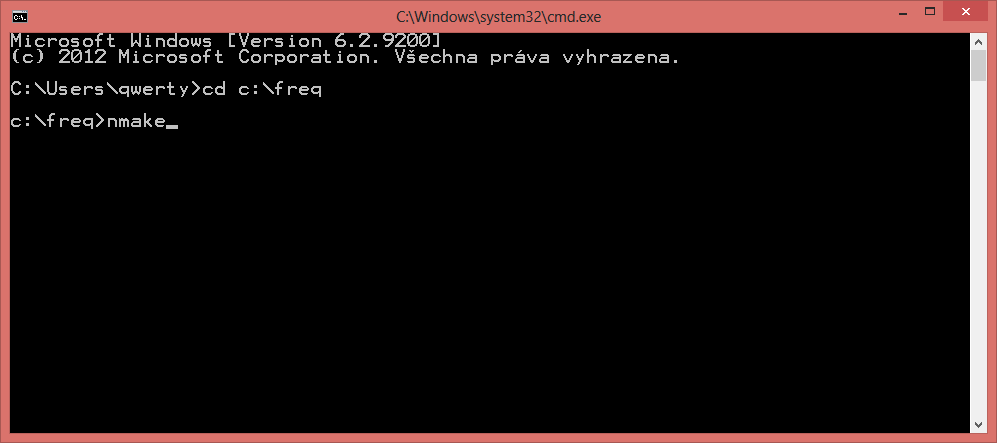
\includegraphics[width=.90\textwidth]{pics/windows.png}
  \caption{Příkazový řádek v systému Windows 8.}
  \label{fig:windowscommand}
\end{figure}
%
\subsubsection{Linux}
%
Nejdříve si spustíme Terminál. Postup se liší podle distribuce Linuxu, ve většině
případů lze terminál najít menu s aplikacemi na systémové liště. Jak vypadá terminál 
je možné vidět na obrázku \ref{fig:linuxterminal}. V Terminálu se
příkazem \texttt{cd} \textit{<složka s rozbalenými soubory>} přeneseme do složky, kam jsme 
si program rozbalili. Překlad provedeme příkazem \texttt{make}, spuštění pak příkazem 
\texttt{./freq.exe} \textit{<soubor-s-vysílači>}.

\begin{figure}[htbp]
  \centering
    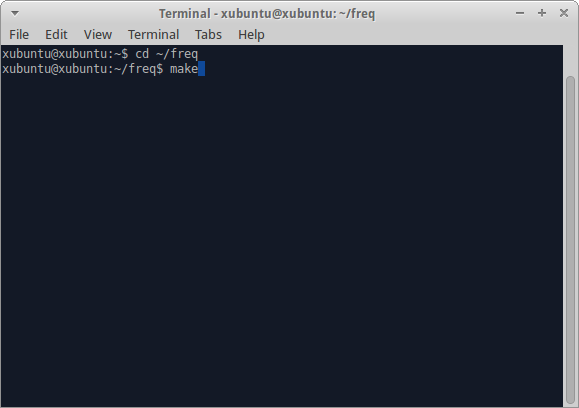
\includegraphics[width=.75\textwidth]{pics/linux.png}
  \caption{Terminál v systému Xubuntu 14.04.}
  \label{fig:linuxterminal}
\end{figure}
%
\newpage
\section{Závěr}
%
O jazyce C jsem vždy smýšlel jako o atomovém výbuchu v \texttt{ASCII-artu} a 
nikdy jsem se nemohl v těch hvězdičkách, ampersandech a šipkách vyznat. Dříve jsem 
si napsal program v C využívající knihovnu \texttt{SDL}, který ze vstupu sbíral názvy zvukových
souborů, které následně přehrával. Zdrojový kód vznikl spíše slepením více \textit{examplů} z internetu, a nějak jsem se divil,
proč program během svého běhu zabírá čím dál více prostoru v paměti. Až v průběhu tohoto 
předmětu mi došlo, jak bláhový jsem byl při psaní onoho kódu. 

Během pár hodin předmětu jsem se naučil stokrát víc, než během stovek hodin 
samostudia, kdy jsem se snažil proniknout do tajů \uv{Céčka}. 
Myslím, že už konečně rozumím pointerům, které mi dříve dělali velké problémy.

Zároveň si velmi cením toho, že jsem byl donucen seznámit se systémem \LaTeX, 
čehož jistě v budoucnu využiji.
%
%
\end{document}